% Decision guide for the use of calibration (Discussion). pdflatex fig_decision; copy to ../figures.
\documentclass[tikz,border=3pt]{standalone}
\usepackage[T1]{fontenc}
\usepackage[scaled=0.92]{helvet}
\renewcommand{\familydefault}{\sfdefault}
\usepackage{sansmath}\sansmath
\usetikzlibrary{positioning,arrows.meta,shapes.geometric,shadows.blur}
\definecolor{ink}{HTML}{1F2328}\definecolor{ink2}{HTML}{57606A}\definecolor{ink3}{HTML}{8C959F}
\definecolor{cQ}{HTML}{2A78D6}\definecolor{cY}{HTML}{1A9E6F}\definecolor{cN}{HTML}{8C959F}
\tikzset{
 q/.style={rounded corners=10pt, draw=cQ, fill=cQ!8, line width=0.9pt, text width=3.45cm, align=center, font=\footnotesize, minimum height=1.25cm, inner sep=4pt, blur shadow={shadow blur steps=5, shadow opacity=15}},
 go/.style={rounded corners=3pt, draw=cY, fill=cY!12, line width=1pt, text width=3.45cm, align=center, font=\footnotesize\bfseries, minimum height=1.1cm, inner sep=4pt, blur shadow={shadow blur steps=5, shadow opacity=15}},
 stop/.style={rounded corners=3pt, draw=cN, fill=white, line width=0.7pt, text width=3.45cm, align=center, font=\footnotesize, text=ink, minimum height=0.95cm, inner sep=4pt},
 a/.style={-{Stealth[length=6pt]}, line width=1.1pt, color=ink3},
 lab/.style={font=\scriptsize\bfseries, fill=white, inner sep=1.5pt},
}
\begin{document}
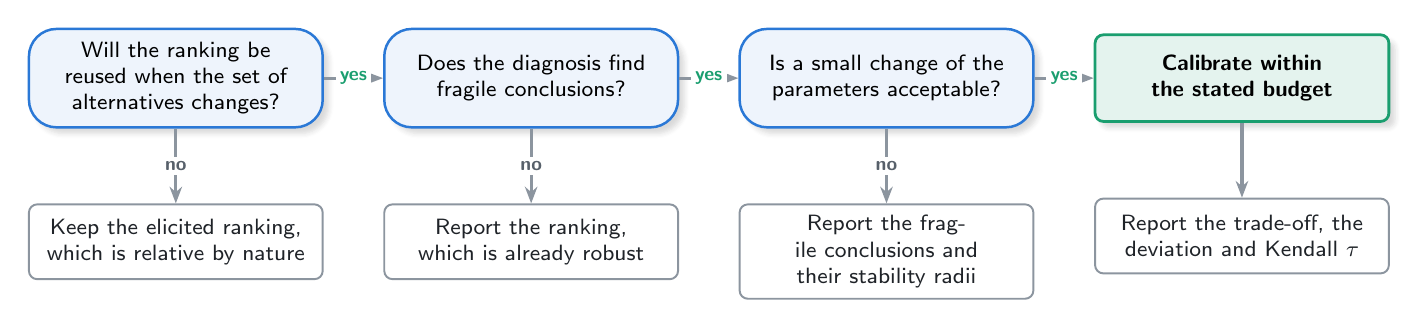
\begin{tikzpicture}[node distance=0.95cm and 0.75cm]
\node[q] (q1) {Will the ranking be reused when the set of alternatives changes?};
\node[q, right=of q1] (q2) {Does the diagnosis find fragile conclusions?};
\node[q, right=of q2] (q3) {Is a small change of the parameters acceptable?};
\node[go, right=of q3] (go) {Calibrate within the stated budget};
\node[stop, below=of q1] (s1) {Keep the elicited ranking, which is relative by nature};
\node[stop, below=of q2] (s2) {Report the ranking, which is already robust};
\node[stop, below=of q3] (s3) {Report the fragile conclusions and their stability radii};
\node[stop, below=of go] (s4) {Report the trade-off, the deviation and Kendall $\tau$};
\draw[a] (q1) -- node[lab, text=cY] {yes} (q2);
\draw[a] (q2) -- node[lab, text=cY] {yes} (q3);
\draw[a] (q3) -- node[lab, text=cY] {yes} (go);
\draw[a] (q1) -- node[lab, text=ink2] {no} (s1);
\draw[a] (q2) -- node[lab, text=ink2] {no} (s2);
\draw[a] (q3) -- node[lab, text=ink2] {no} (s3);
\draw[a] (go) -- (s4);
\end{tikzpicture}
\end{document}
